\begin{figure}[tbp]
\centering
\begin{tikzpicture}[x=1cm,y=1cm,>=stealth,font=\small,
  first/.style={draw=blue!65!black,line width=.85pt},
  second/.style={draw=orange!80!black,line width=.85pt}]
  \begin{scope}
    \draw[gray!65] (0,0) circle (.85);
    \draw[first,->] (-.85,0)--(.85,0);
    \draw[second,->] (0,-.85)--(0,.85);
    \node[below right] at (.57,0) {$C$};
    \node[above right] at (0,.62) {$E$};
    \node at (0,-1.17) {$(C,E):\ +1$};
  \end{scope}
  \begin{scope}[xshift=3.25cm]
    \draw[gray!65] (145:.85) arc (145:35:.85);
    \draw[first,->] (0,.85)--(0,1.55);
    \draw[second,dashed,->] (.23,.8185)--(.23,1.55);
    \fill[blue!65!black] (0,.85) circle (1.7pt);
    \fill[orange!80!black] (.23,.8185) circle (1.7pt);
    \node at (0,-.02) {$T=-1$};
    \node at (0,-.45) {right shift};
    \node[above] at (0,1.63) {same spoke};
  \end{scope}
  \begin{scope}[xshift=6.5cm]
    \draw[gray!65] (145:.85) arc (145:35:.85);
    \draw[first,->] (0,.85)--(0,1.55);
    \draw[second,dashed,->] (-.23,.8185)--(-.23,1.55);
    \fill[blue!65!black] (0,.85) circle (1.7pt);
    \fill[orange!80!black] (-.23,.8185) circle (1.7pt);
    \node at (0,-.02) {$T=+1$};
    \node at (0,-.45) {left shift};
    \node[above] at (0,1.63) {same spoke};
  \end{scope}
  \node at (4.875,-1.17) {average: $\tfrac12(-1+1)=0$};
\end{tikzpicture}
\caption{The local signs in the cycle pairing. Left: a chord directed to
the right followed by one directed upward gives a positive crossing.
Right: alternative right and left displacements of the second track at
a shared spoke give opposite comparisons in counterclockwise boundary
order. The two displacements are alternative perturbations whose counts are averaged.}
\label{fig:local-pairing}
\end{figure}
